\documentclass[10pt,twocolumn]{article}
\usepackage{geometry}
\geometry{verbose,headsep=3cm,tmargin=2.5cm,bmargin=2.5cm,lmargin=2.0cm,rmargin=2.0cm}
\usepackage{graphicx}
\usepackage{xcolor}
\usepackage[font=small]{caption}
\usepackage{amsmath,amssymb,latexsym}
\usepackage{marvosym}
\usepackage{url}
\usepackage{lipsum}
\usepackage{bm}
\usepackage{float}
\usepackage[english]{babel}
\usepackage{caption}
%\usepackage{subfigure}
\usepackage{subcaption}
\usepackage{subfloat}
\usepackage{hyperref}
\usepackage{epsf}
\usepackage{float}
\usepackage{mathpazo}
\usepackage{pifont}
\usepackage{graphicx}
%\usepackage{subfig}
\usepackage{wrapfig}
\usepackage{multicol}
\usepackage{enumitem}
\usepackage{xcolor}
\usepackage{framed}
\usepackage[utf8]{inputenc}
% Document font:
\usepackage{charter}
\graphicspath{{DWGs/}}
\newcommand*{\addheight}[2][.5ex]{%
  \raisebox{0pt}[\dimexpr\height+(#1)\relax]{#2}%
}

\begin{document}

\twocolumn[{
\begin{@twocolumnfalse}

  \begin{center}
%\textcolor{lgray}
    \vskip-5em

    \hfill
    \fontsize{10}{10}\selectfont {\textit{Bruxelles, January 2019}}

    \vskip2ex
    
	\vspace{5ex}
	
    \fontsize{24}{10}\selectfont {Underdetermined linear systems}
    
    \fontsize{18}{10}\selectfont {a short story with some code}



  \noindent%
    
\vskip1ex

{\rule{\textwidth}{0.5pt}}

  \end{center}
  
    \fontsize{7}{10}\selectfont {This work is licensed under the Creative Commons Attribution-NonCommercial-ShareAlike 4.0 International (CC BY-NC-SA 4.0) license.}

\vspace{6mm}

\end{@twocolumnfalse}
}]

\setlength{\parindent}{0cm}

\vspace{10mm}

\setlength{\parindent}{0cm}

\fontsize{14}{10}\selectfont {Kamila Zdybał}

\vspace{2mm}

\fontsize{8}{10}\selectfont {\textit{Université libre de Bruxelles, kamila.zdybal@ulb.ac.be}}

\fontsize{8}{10}\selectfont {\textit{camillejr.github.io/science-docs, kamila.zdybal@gmail.com}}

\vspace{2mm}



\section*{Preface}



\,\,

This document is still in preparation. Please feel free to contact me with any suggestions, corrections or comments.

\section*{Keywords}

\textit{underdetermined linear systems, linear algebra, matrix decomposition, matrix approximation}

\tableofcontents

\section{Introduction}

For an undertermined linear system (where matrix $\bm{A}$ is size $(n \times m)$ and $n<m$):

\begin{equation}
\bm{A} x = b
\end{equation}


an infinite number of solutions exists. MATLAB implements various methods of computing possible solutions for $x$. In this paper we investigate the differences in the available solutions by analyzing their histograms. Four methods were selected: backslash \texttt{\char`\\} operator, computing a pseudo-inverse \texttt{pinv()}, and two least-squares algorithms \texttt{lsqnonneg()} and \texttt{lsqr()}.

\section{Matlab example}

We focus on an example where matrix $\bm{A}$ is size $(100 \times 500)$ and a vector $b$ is size $(100 \times 1)$; both are populated by normally distributed random numbers.

\begin{figure}[H]
\centering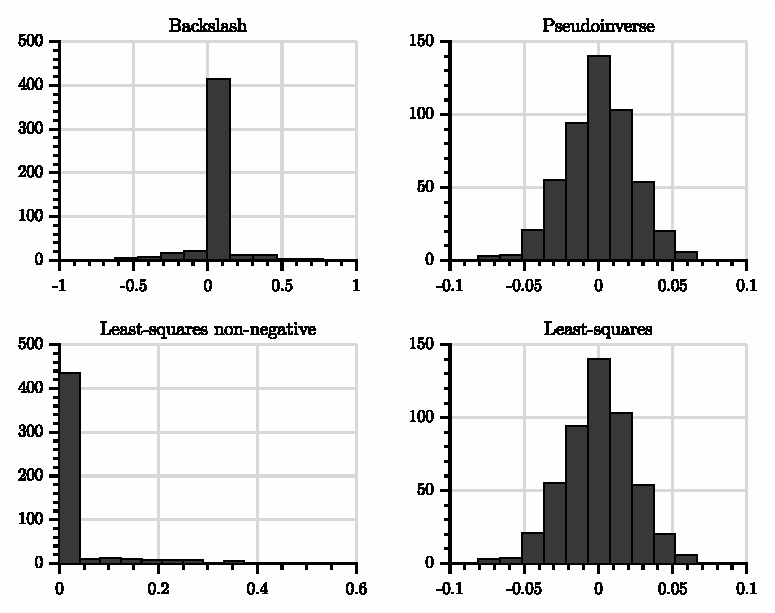
\includegraphics[width=8cm]{DWGs/histograms.eps}
\caption{Histograms of four solutions to an undetermined linear system.}			
\label{fig:histograms}
\end{figure}







\section{Possible applications}


\newpage

\section{Low-rank approximations}

We perform Principal Component Analysis (PCA) on three generated matrices of size $(10 \times 6)$: a random matrix which is populated by random floats in the range 0-1 and a semi-structured and structured matrices whose elements are also in the range 0-1 but were populated by the user and have an increasing level of structure that was judged visually. These matrices are presented in Fig. \ref{fig:matrices}.

\begin{figure}[H]
\begin{subfigure}[t]{.15\textwidth}
\centering
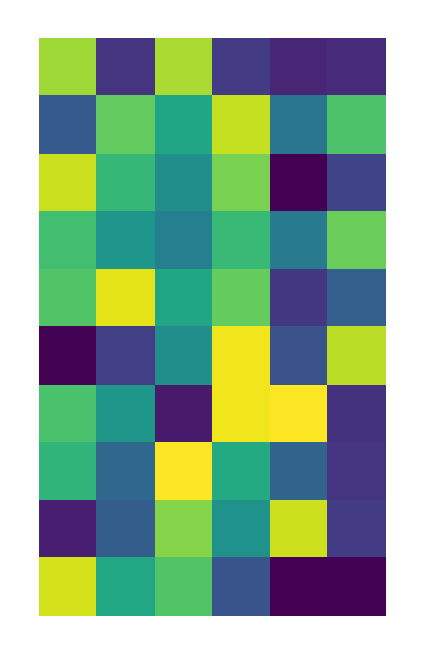
\includegraphics[scale=.2]{DWGs/random-matrix-original.eps}
\caption{ }
\end{subfigure}
\begin{subfigure}[t]{.15\textwidth}
\centering
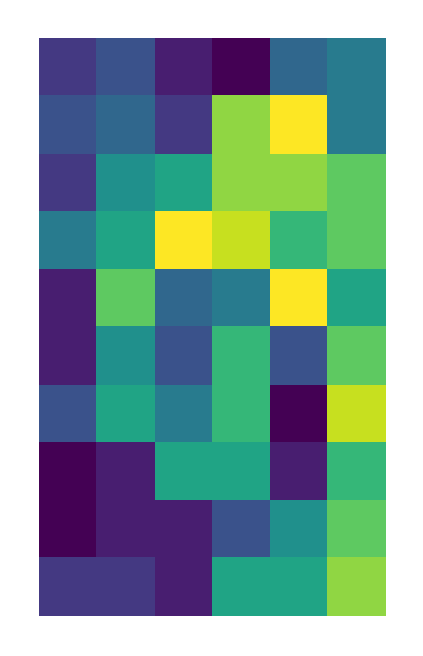
\includegraphics[scale=.2]{DWGs/semi-structured-matrix-original.eps}
\caption{ }
\end{subfigure}
\begin{subfigure}[t]{.15\textwidth}
\centering
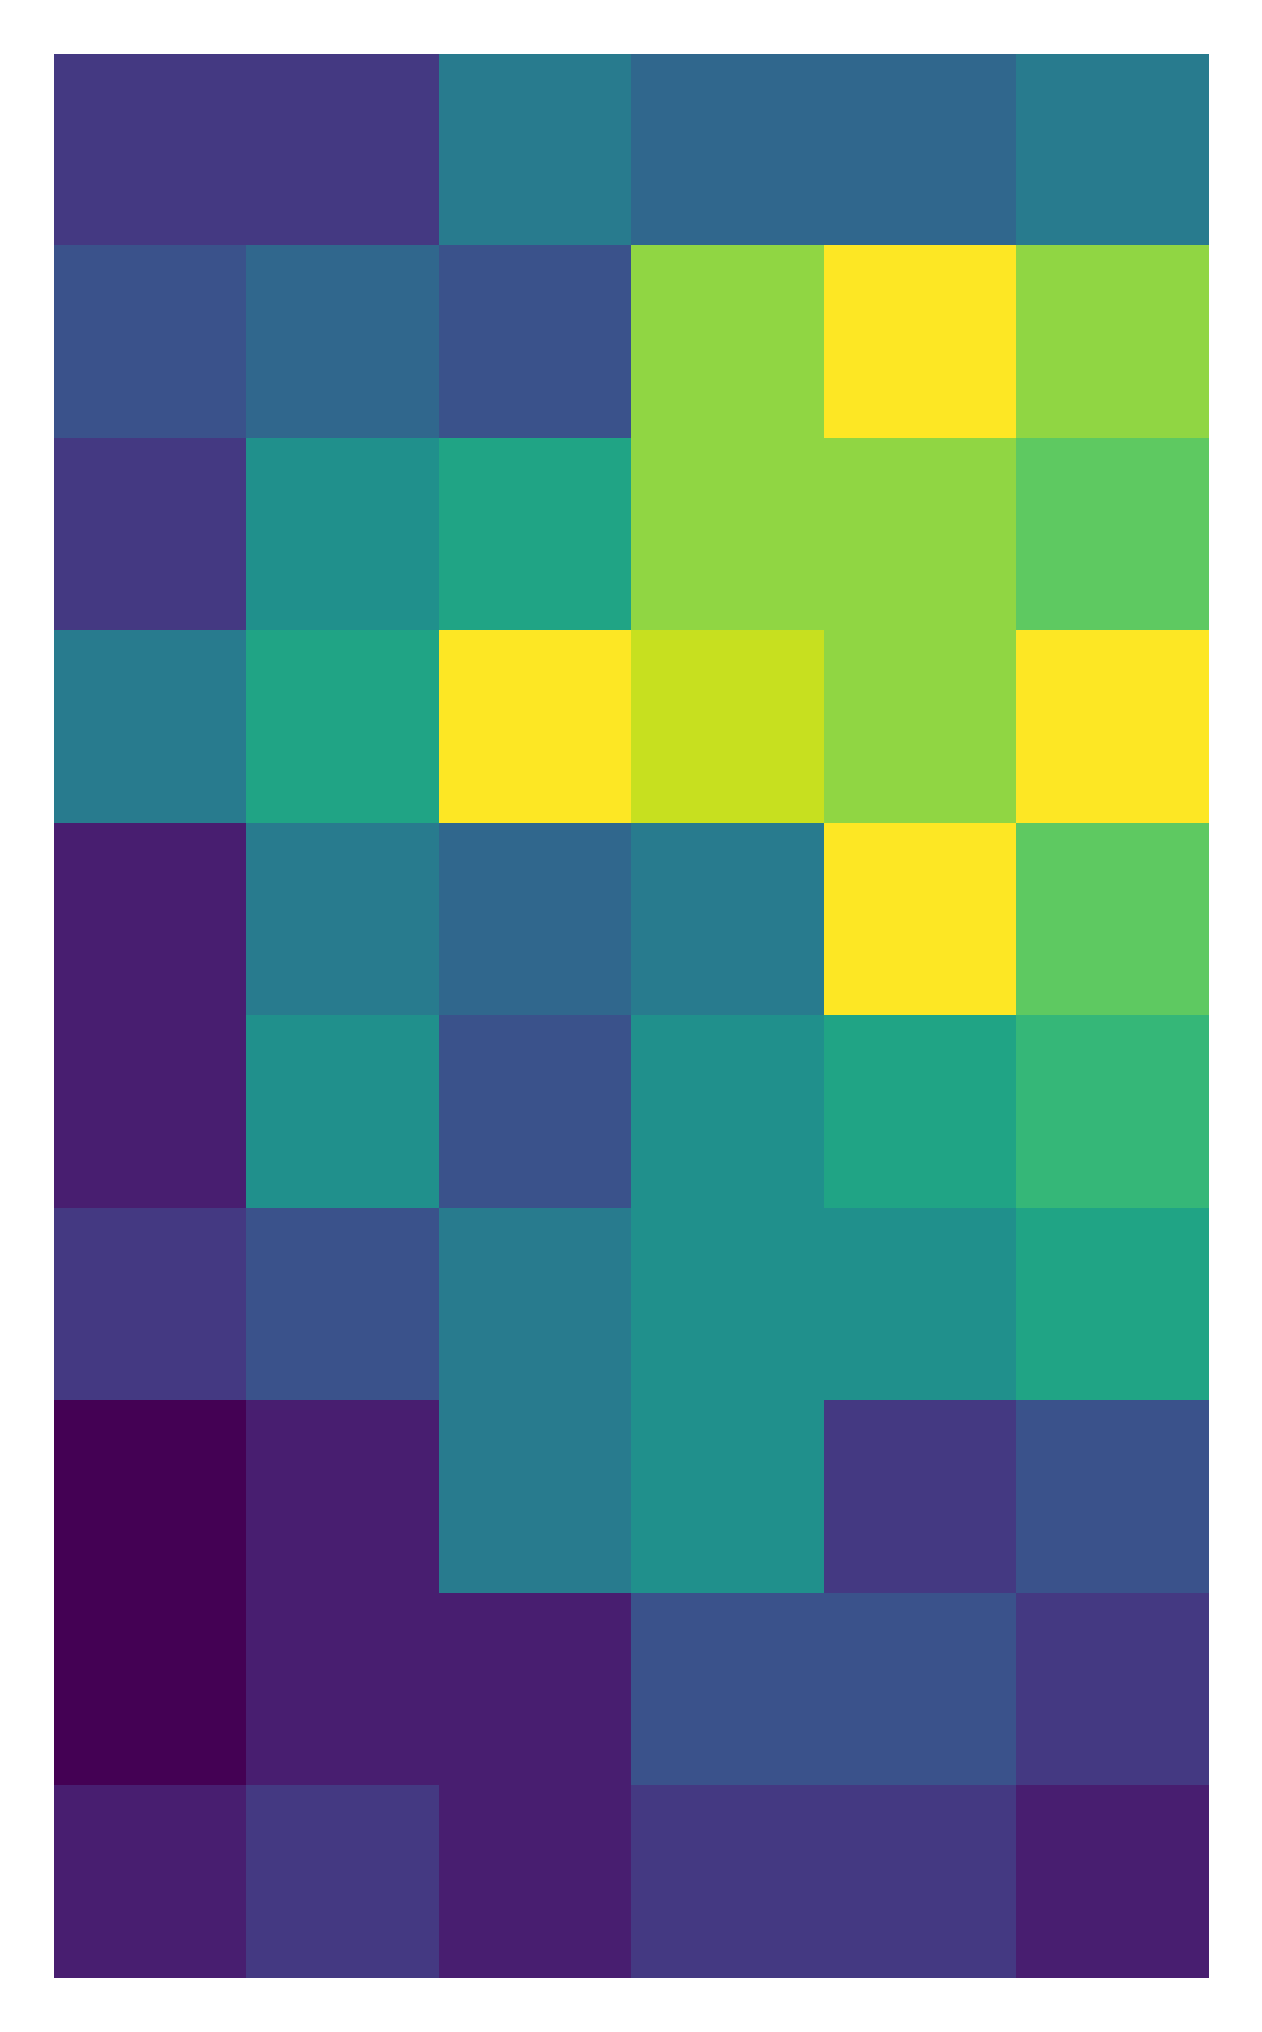
\includegraphics[scale=.2]{DWGs/structured-matrix-original.eps}
\caption{ }
\end{subfigure}
\caption{Original matrices: (a) random matrix, (b) semi-structured matrix, (c) structured matrix.}
\label{fig:matrices}
\end{figure}

The visual judgment of the level of imposed "structure" is quite objective but the aim was to group the elements of high numerical value (most yellow) in a single region of the matrix and elements of low numerical (most purple) value in other regions of the matrix.

The level of the imposed "structure" can also be observed quantitatively after performing PCA from the eigenvalue distribution, presented in Fig. \ref{fig:eigenvalues}. The structured matrix has got the strongest decaying behaviour which suggest that the matrix can be approximated by relatively low number of modes and hence exhibits a strong low-rank structure. The first Principal Component (PC) is expected to carry 80\% of the total variance in the structured data matrix.

\begin{figure}[H]
\centering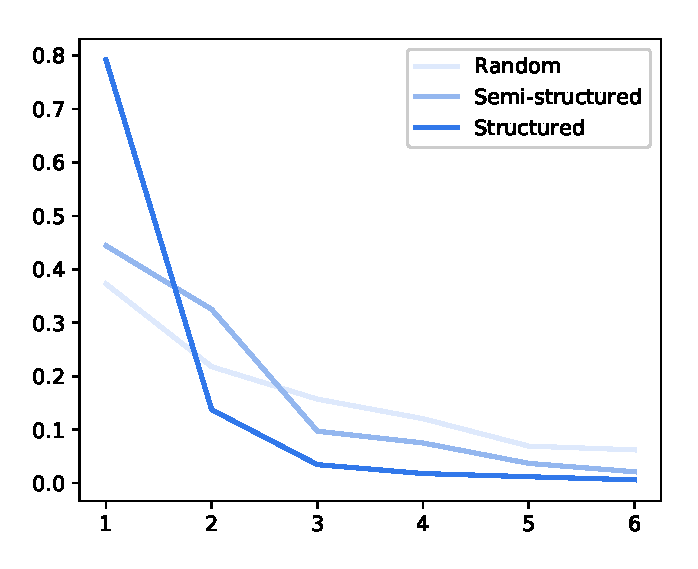
\includegraphics[width=6cm]{DWGs/matrix-reconstruction-eigenvalues-comparison.eps}
\caption{Eigenvalues distribution after performing PCA on data matrices.}			
\label{fig:eigenvalues}
\end{figure}

We may reconstruct the original data matrices using a certain number $q$ of PC-scores and corresponding PCs. Using the Matlab notation we may write the approximation as:

\begin{equation}
\bm{D}_{\text{app}} = \text{PC-scores}(:,1:q) \cdot \text{PCs}(1:q,:)
\end{equation}

Below we can see a rank-1 approximation of the original matrices using the $1^{st}$ Principal Component found by PCA. The vectors $(10 \times 1)$ represent the PC-scores and the vectors $(1 \times 6)$ represent the PCs.

What can be seen visually is that for the semi-structured and structured matrix the low numerical value region is clearly separated. For the random matrix, only few regions of lowest and highest numerical values are visible in the rank-1 approximation.

\begin{figure}[H]
\begin{subfigure}[t]{.15\textwidth}
\centering
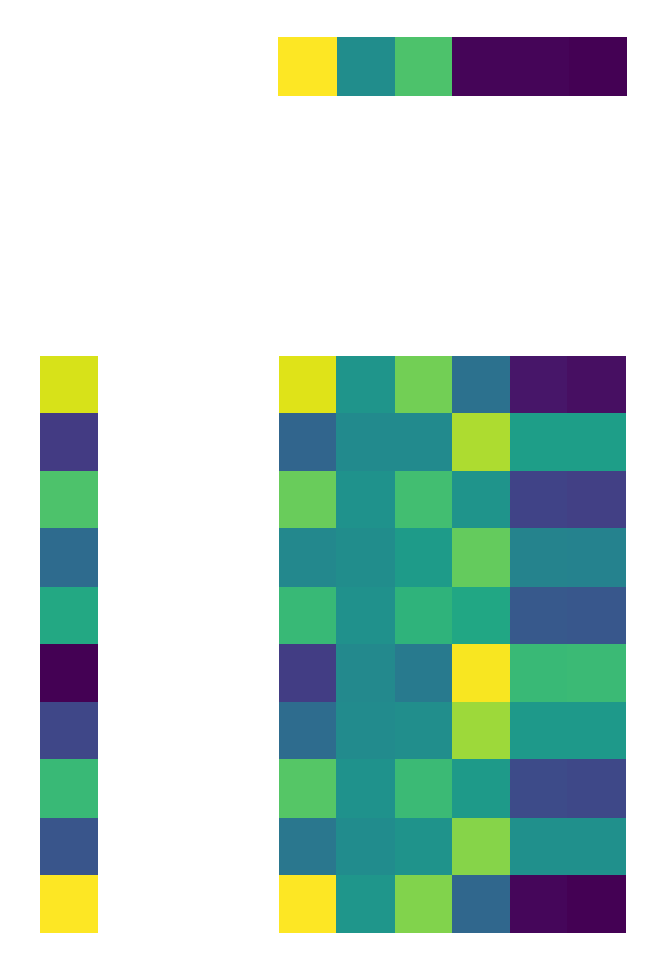
\includegraphics[scale=.2]{DWGs/random-matrix-reconstruction-PCs-1.eps}
\caption{ }
\end{subfigure}
\begin{subfigure}[t]{.15\textwidth}
\centering
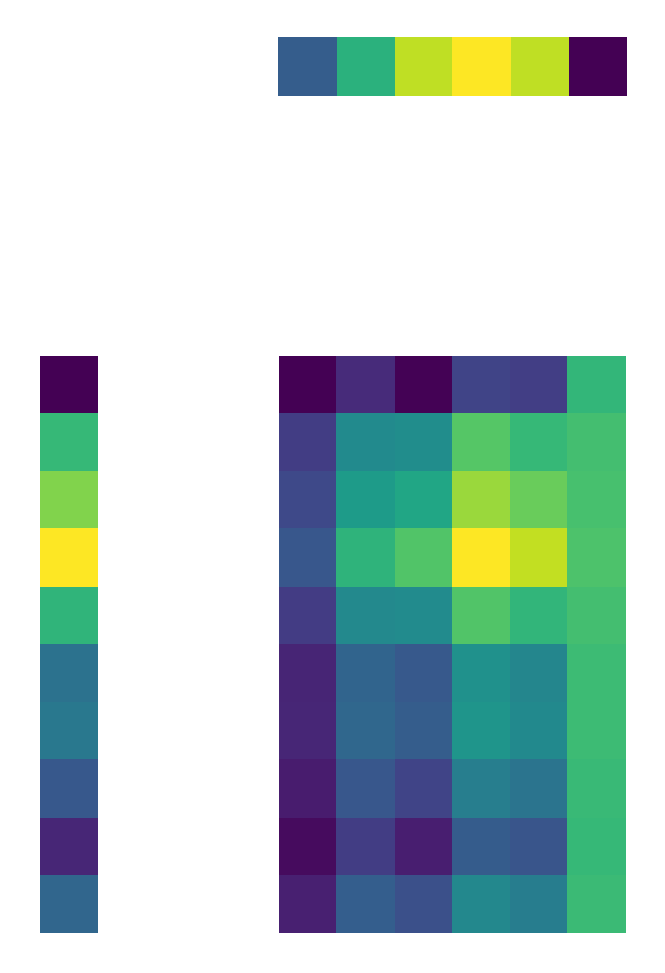
\includegraphics[scale=.2]{DWGs/semi-structured-matrix-reconstruction-PCs-1.eps}
\caption{ }
\end{subfigure}
\begin{subfigure}[t]{.15\textwidth}
\centering
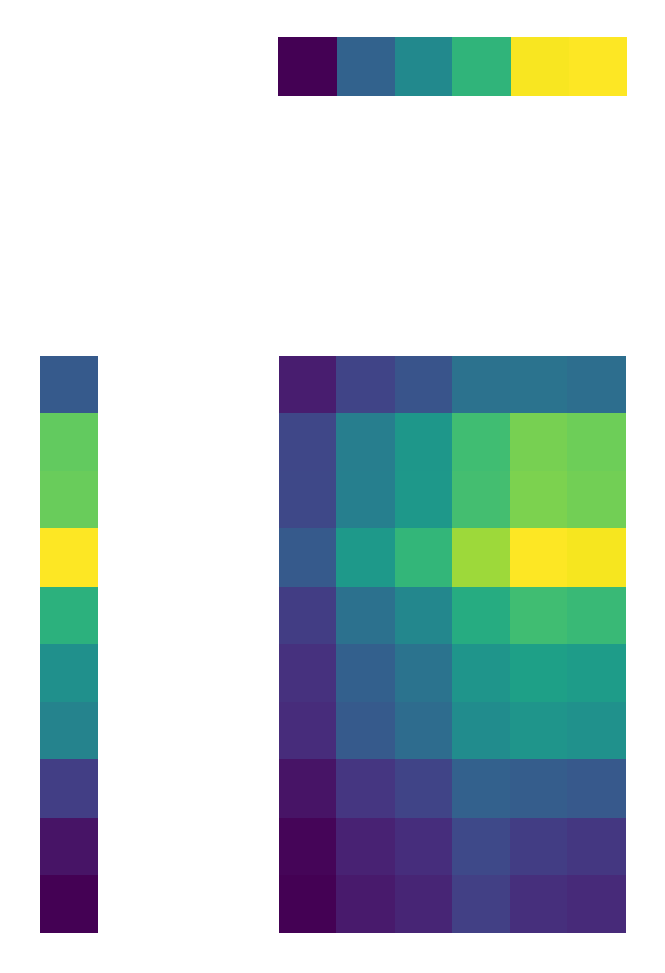
\includegraphics[scale=.2]{DWGs/structured-matrix-reconstruction-PCs-1.eps}
\caption{ }
\end{subfigure}
\caption{PCA reconstruction with $1^{st}$ Principal Component of: (a) random matrix, (b) semi-structured matrix, (c) structured matrix.}
\label{fig:matrices-reconstruction}
\end{figure}

In Fig. \ref{fig:matrices-reconstruction} we present a rank-2 approximation, where we took two PCs. Again, the matrix $(10 \times 2)$ represent the PC-scores and the vectors $(2 \times 6)$ represent the PCs.

In the semi-structured and structured matrix, the single matrix elements with highest numerical values (yellow) are already recovered in their actual positions. In the random matrix this is still not the case with rank 2-approximation.

\begin{figure}[H]
\begin{subfigure}[t]{.15\textwidth}
\centering
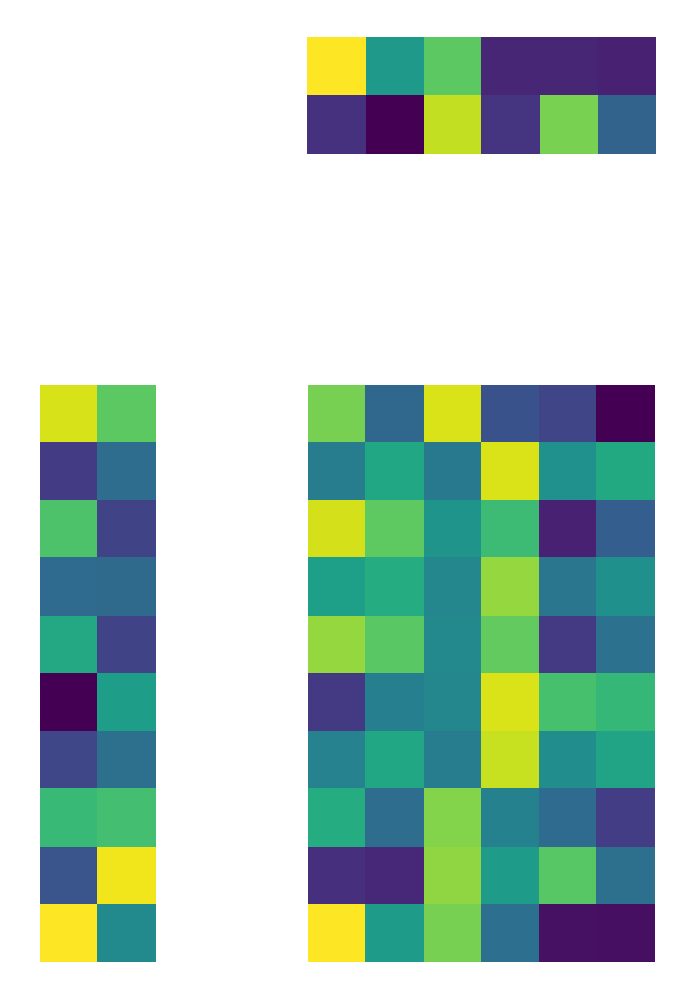
\includegraphics[scale=.2]{DWGs/random-matrix-reconstruction-PCs-2.eps}
\caption{ }
\end{subfigure}
\begin{subfigure}[t]{.15\textwidth}
\centering
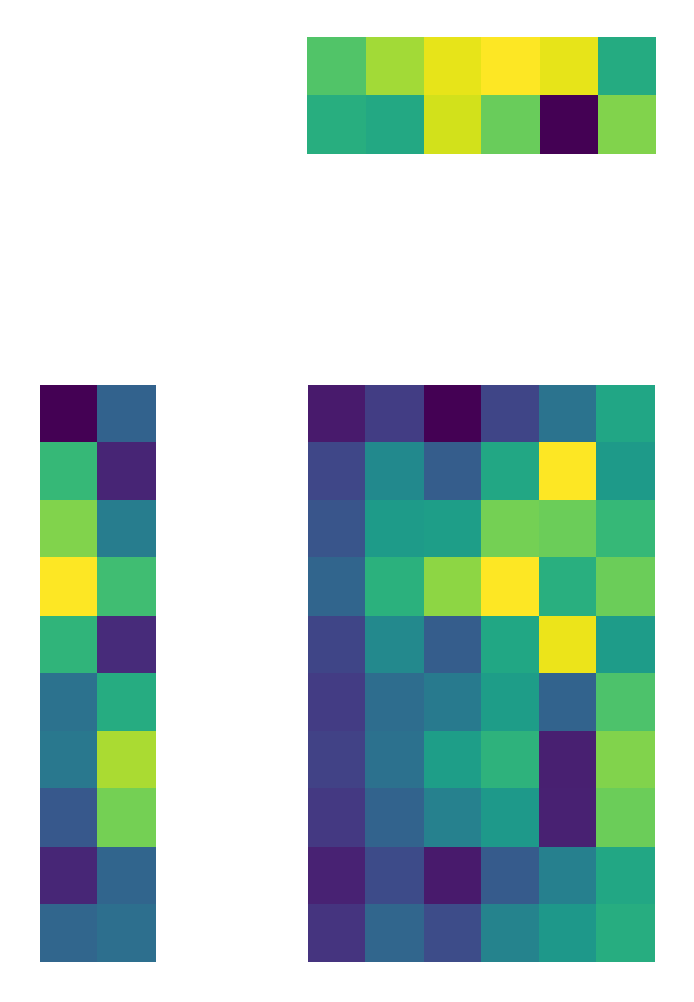
\includegraphics[scale=.2]{DWGs/semi-structured-matrix-reconstruction-PCs-2.eps}
\caption{ }
\end{subfigure}
\begin{subfigure}[t]{.15\textwidth}
\centering
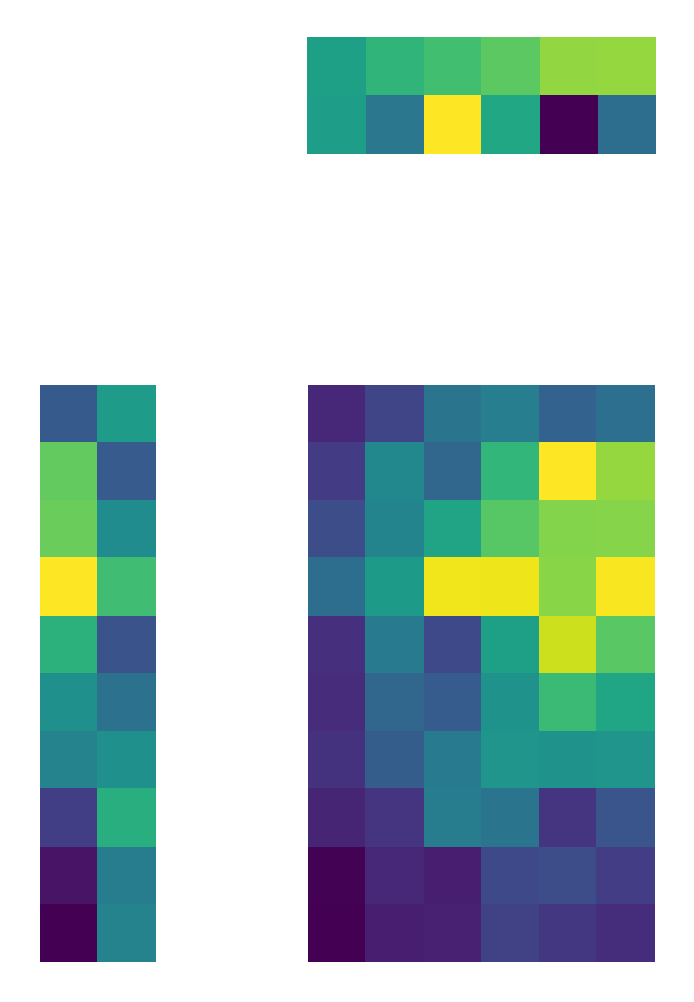
\includegraphics[scale=.2]{DWGs/structured-matrix-reconstruction-PCs-2.eps}
\caption{ }
\end{subfigure}
\caption{PCA reconstruction with 2 Principal Components of: (a) random matrix, (b) semi-structured matrix, (c) structured matrix.}
\label{fig:matrices-reconstruction}
\end{figure}



The original data matrices are not completely retrieved until all 6 Principal Components and 6 PC-scores are taken into account. We obtain the final data matrices of rank-6.

\begin{figure}[H]
\begin{subfigure}[t]{.15\textwidth}
\centering
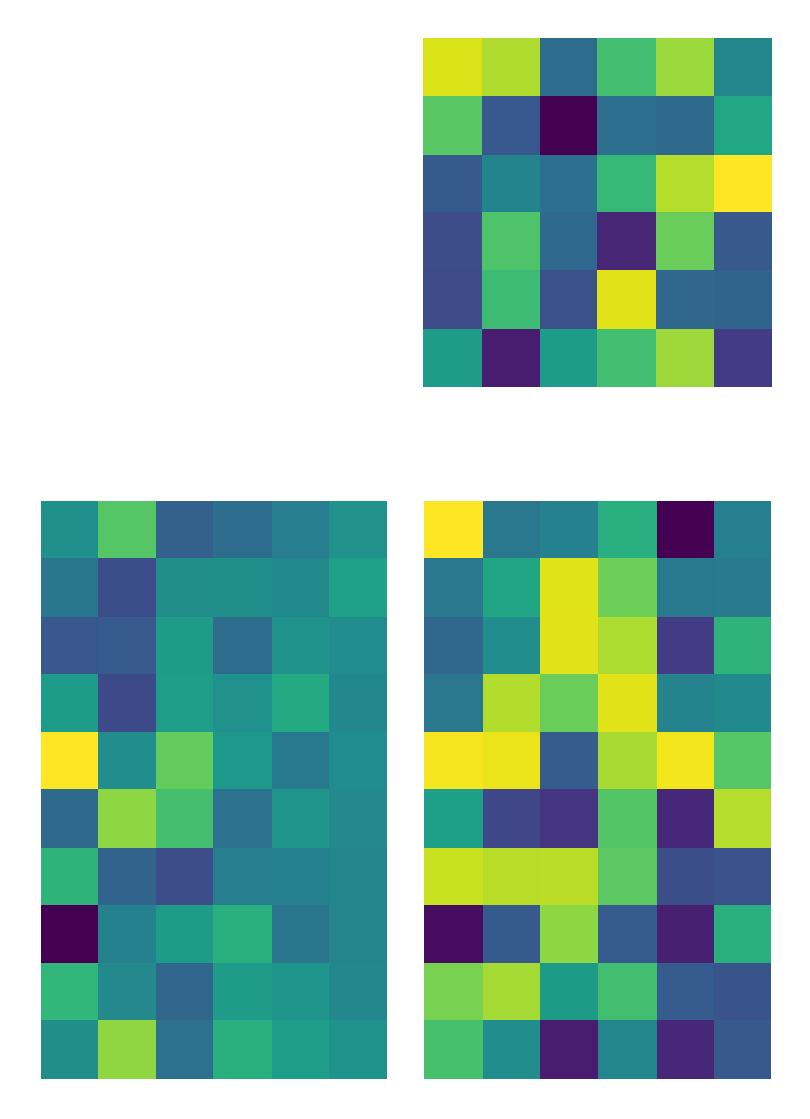
\includegraphics[scale=.2]{DWGs/random-matrix-reconstruction-PCs-6.eps}
\caption{ }
\end{subfigure}
\begin{subfigure}[t]{.15\textwidth}
\centering
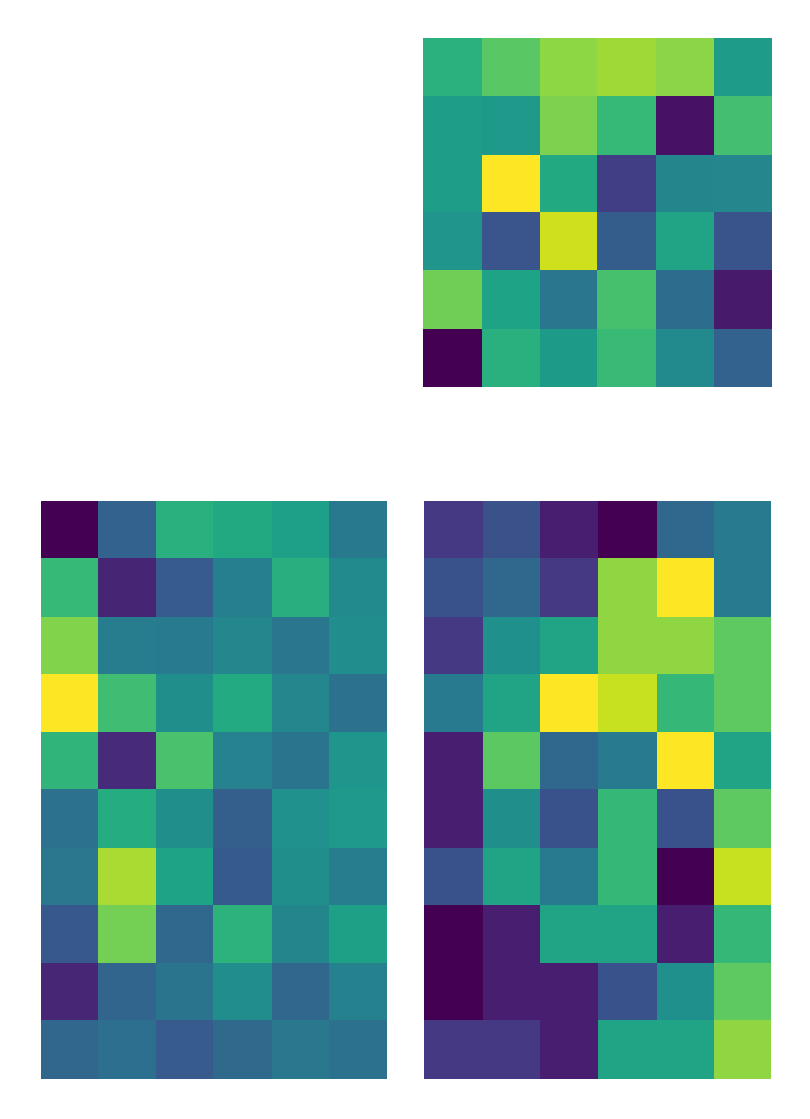
\includegraphics[scale=.2]{DWGs/semi-structured-matrix-reconstruction-PCs-6.eps}
\caption{ }
\end{subfigure}
\begin{subfigure}[t]{.15\textwidth}
\centering
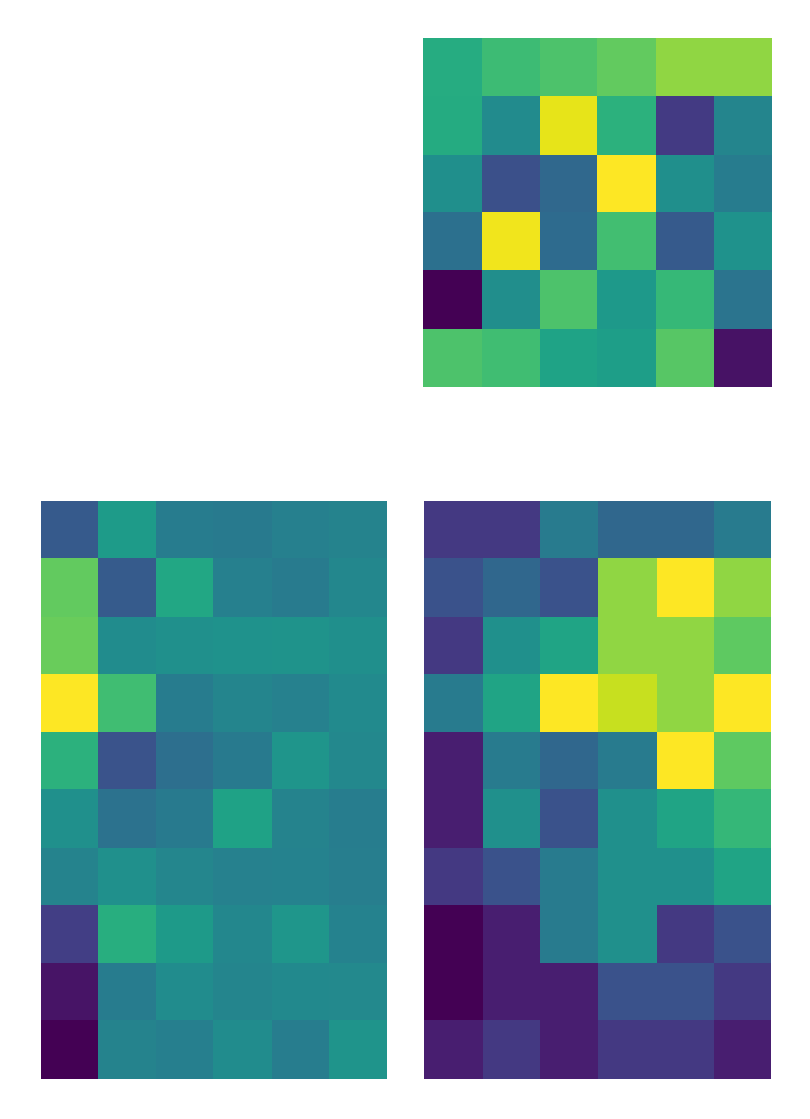
\includegraphics[scale=.2]{DWGs/structured-matrix-reconstruction-PCs-6.eps}
\caption{ }
\end{subfigure}
\caption{PCA reconstruction with 6 Principal Components of: (a) random matrix, (b) semi-structured matrix, (c) structured matrix.}
\label{fig:matrices-reconstruction}
\end{figure}


\thebibliography{}

\bibitem{Kutz} Nathan Kutz, \textit{Data Driven Discovery of Dynamical Systems and PDEs}, an online lecture 

\bibitem{Strang} Gilbert Strang, \textit{Introduction to Linear Algebra}, Fifth Edition, 2016

 \label{bib:pope}


\end{document}
